\subsection{Post-trained Language Model}
\label{section:results_finetuned}

We present results for our \llamathree post-trained models on benchmarks across different capabilities.
Similar to pre-training we are releasing the data generated as part of evaluations with publicly available benchmarks which can be found on \href{https://huggingface.co/meta-llama}{Huggingface here}. Additional details on our eval setup can be found \href{https://github.com/meta-llama/llama-models/blob/main/models/llama3_1/eval_details.md}{here}.

\begin{table}
    \centering
    \begin{tabular}{ll}
    \toprule   
    \makecell[l]{\textbf{General}} & \makecell[l]{
        MMLU \citep{hendrycks2021mmlu}, MMLU-Pro \citep{wang2024mmlu}, \\ 
        IFEval \citep{zhou2023instruction} \\
    }\\
    \midrule
    \makecell[l]{\textbf{Math and reasoning}} & \makecell[l]{
        GSM8K \citep{cobbe2021training}, MATH \citep{hendrycks2021measuring},\\ GPQA \citep{rein2023gpqagraduatelevelgoogleproofqa},  ARC-Challenge \citep{clark2018think}\\
    }\\
    \midrule
    \makecell[l]{\textbf{Code}} & \makecell[l]{
        HumanEval \citep{chen2021evaluating}, MBPP \citep{austin2021program},\\ HumanEval+~\citep{liu2024your}, MBPP EvalPlus (base) \citep{liu2024your}, \\ MultiPL-E~\citep{cassano2022multiple}
    }\\
    \midrule
    \makecell[l]{\textbf{Multilinguality}} & \makecell[l]{
    MGSM \citep{shi2022languagemodelsmultilingualchainofthought}, Multilingual MMLU (internal benchmark) 
    }\\
    \midrule
    \makecell[l]{\textbf{Tool-use}} & \makecell[l]{
    Nexus~\citep{srinivasan2023nexusraven}, API-Bank~\citep{li2023api}, \\API-Bench~\citep{patil2023gorilla}, BFCL~\citep{berkeley-function-calling-leaderboard}
    }\\
    \midrule
    \makecell[l]{\textbf{Long context}} & \makecell[l]{
        ZeroSCROLLS \citep{zeroscrolls},
        Needle-in-a-Haystack \citep{niah},\\
        InfiniteBench \citep{zhang2024infty}
    }\\
\bottomrule
\end{tabular}

    \caption{\textbf{Post-training benchmarks by category.} Overview of all benchmarks we use to evaluate post-trained \llamathree models, ordered by capability. %
    }
    \label{table:posttraining_benchmarks}
\end{table}

\textbf{Benchmarks and metrics.} Table~\ref{table:posttraining_benchmarks} contains an overview of all the benchmarks, organized by the capability.
We apply decontamination of the post-training data by running exact match with the prompts from each benchmark. In addition to the standard academic benchmarks, we also performed extensive human evaluation of different capabilities. Details are provided in Section~\ref{section:human_evals}.

\textbf{Experimental setup.} We employ a similar experimental setup to the pre-training phase and conduct a comparative analysis of \llamathree alongside other models of comparable size and capability. To the extent possible, we evaluate the performance of other models ourselves and compare the results with the reported numbers, selecting the best score.
You can find additional details on our evaluation setup \href{https://github.com/meta-llama/llama-models/blob/main/models/llama3_1/eval_details.md}{here}.

\subsubsection{General Knowledge and Instruction-Following Benchmarks}
We evaluate \llamathree on benchmarks for general knowledge and instruction-following in Table~\ref{table:the_major_result_table}.

\textbf{General knowledge.} We leverage MMLU~\citep{hendrycks2021mmlu} and MMLU-Pro~\citep{wang2024mmlu} to evaluate \llamathree's capability on knowledge-based question answering. For MMLU, we report the macro average of subtask accuracy under the 5-shot standard setting without CoT. MMLU-Pro is an extension of MMLU, incorporating more challenging, reasoning-focused questions, eliminating noisy questions, and expanding the choice set from four to ten options. Given its focus on complex reasoning, we report 5-shot CoT for MMLU-Pro. All tasks are formatted as generation tasks, similar to simple-evals~\citep{simpleevals}.

As shown in Table~\ref{table:the_major_result_table}, our 8B and 70B \llamathree variants outperform other models of similar sizes on both general knowledge tasks. Our 405B model outperforms \gptp and \nemotron, with \sonnet leading among larger models.


\textbf{Instruction following.} We assess the ability of \llamathree and other models to follow natural language instructions on IFEval ~\citep{zhou2023instruction}. IFEval comprises approximately 500 ``verifiable instructions'' such as ``write in more than 400 words'', which can be verified by heuristics. We report the average of prompt-level and instruction-level accuracy, under strict and loose constraints in Table~\ref{table:the_major_result_table}. Note that all \llamathree variants outperform comparable models across IFEval.

\begin{table*}[t]
    \centering
    \begin{NiceTabular}{lccccccc}
    \CodeBefore
    \Body
    \toprule
          \textbf{Exam}    & \rotate\textbf{\llamathree 8B} & \rotate\textbf{\llamathree 70B} & \rotate\textbf{\llamathree 405B} & \rotate\textbf{\gptthreedotfivet} & \rotate\textbf{\nemotron} & \rotate\textbf{\gpto} & \rotate\textbf{\sonnet} \\
    \midrule
    LSAT & 53.9 \scriptsize{$\pm$4.9} & 74.2 \scriptsize{$\pm$4.3} & \textbf{81.1 \scriptsize{$\pm$3.8}} & 54.3 \scriptsize{$\pm$4.9} & 73.7 \scriptsize{$\pm$4.3} & 77.4 \scriptsize{$\pm$4.1} & 80.0 \scriptsize{$\pm$3.9} \\
SAT Reading & 57.4 \scriptsize{$\pm$4.2} & 71.4 \scriptsize{$\pm$3.9} & 74.8 \scriptsize{$\pm$3.7} & 61.3 \scriptsize{$\pm$4.2} & -- & 82.1 \scriptsize{$\pm$3.3} & \textbf{85.1 \scriptsize{$\pm$3.1}} \\
SAT Math & 73.3 \scriptsize{$\pm$4.6} & 91.9 \scriptsize{$\pm$2.8} & 94.9 \scriptsize{$\pm$2.3} & 77.3 \scriptsize{$\pm$4.4} & -- & 95.5 \scriptsize{$\pm$2.2} & \textbf{95.8 \scriptsize{$\pm$2.1}} \\
GMAT Quant. & 56.0 \scriptsize{$\pm$19.5} & 84.0 \scriptsize{$\pm$14.4} & \textbf{96.0 \scriptsize{$\pm$7.7}} & 36.0 \scriptsize{$\pm$18.8} & 76.0 \scriptsize{$\pm$16.7} & 92.0 \scriptsize{$\pm$10.6} & 92.0 \scriptsize{$\pm$10.6} \\
GMAT Verbal & 65.7 \scriptsize{$\pm$11.4} & 85.1 \scriptsize{$\pm$8.5} & 86.6 \scriptsize{$\pm$8.2} & 65.7 \scriptsize{$\pm$11.4} & 91.0 \scriptsize{$\pm$6.8} & \textbf{95.5 \scriptsize{$\pm$5.0}} & 92.5 \scriptsize{$\pm$6.3} \\
GRE Physics & 48.0 \scriptsize{$\pm$11.3} & 74.7 \scriptsize{$\pm$9.8} & 80.0 \scriptsize{$\pm$9.1} & 50.7 \scriptsize{$\pm$11.3} & -- & 89.3 \scriptsize{$\pm$7.0} & \textbf{90.7 \scriptsize{$\pm$6.6}} \\
AP Art History & 75.6 \scriptsize{$\pm$12.6} & 84.4 \scriptsize{$\pm$10.6} & \textbf{86.7 \scriptsize{$\pm$9.9}} & 68.9 \scriptsize{$\pm$13.5} & 71.1 \scriptsize{$\pm$13.2} & 80.0 \scriptsize{$\pm$11.7} & 77.8 \scriptsize{$\pm$12.1} \\
AP Biology & 91.7 \scriptsize{$\pm$11.1} & \textbf{100.0 \scriptsize{$\pm$0.0}} & \textbf{100.0 \scriptsize{$\pm$0.0}} & 91.7 \scriptsize{$\pm$11.1} & 95.8 \scriptsize{$\pm$8.0} & \textbf{100.0 \scriptsize{$\pm$0.0}} & \textbf{100.0 \scriptsize{$\pm$0.0}} \\
AP Calculus & 57.1 \scriptsize{$\pm$16.4} & 54.3 \scriptsize{$\pm$16.5} & 88.6 \scriptsize{$\pm$10.5} & 62.9 \scriptsize{$\pm$16.0} & 68.6 \scriptsize{$\pm$15.4} & \textbf{91.4 \scriptsize{$\pm$9.3}} & 88.6 \scriptsize{$\pm$10.5} \\
AP Chemistry & 59.4 \scriptsize{$\pm$17.0} & \textbf{96.9 \scriptsize{$\pm$6.0}} & 90.6 \scriptsize{$\pm$10.1} & 62.5 \scriptsize{$\pm$16.8} & 68.8 \scriptsize{$\pm$16.1} & 93.8 \scriptsize{$\pm$8.4} & \textbf{96.9 \scriptsize{$\pm$6.0}} \\
AP English Lang. & 69.8 \scriptsize{$\pm$12.4} & 90.6 \scriptsize{$\pm$7.9} & 94.3 \scriptsize{$\pm$6.2} & 77.4 \scriptsize{$\pm$11.3} & 88.7 \scriptsize{$\pm$8.5} & \textbf{98.1 \scriptsize{$\pm$3.7}} & 90.6 \scriptsize{$\pm$7.9} \\
AP English Lit. & 59.3 \scriptsize{$\pm$13.1} & 79.6 \scriptsize{$\pm$10.7} & 83.3 \scriptsize{$\pm$9.9} & 53.7 \scriptsize{$\pm$13.3} & \textbf{88.9 \scriptsize{$\pm$8.4}} & \textbf{88.9 \scriptsize{$\pm$8.4}} & 85.2 \scriptsize{$\pm$9.5} \\
AP Env. Sci. & 73.9 \scriptsize{$\pm$12.7} & 89.1 \scriptsize{$\pm$9.0} & \textbf{93.5 \scriptsize{$\pm$7.1}} & 73.9 \scriptsize{$\pm$12.7} & 73.9 \scriptsize{$\pm$12.7} & 89.1 \scriptsize{$\pm$9.0} & 84.8 \scriptsize{$\pm$10.4} \\
AP Macro Eco. & 72.4 \scriptsize{$\pm$11.5} & \textbf{98.3 \scriptsize{$\pm$3.3}} & \textbf{98.3 \scriptsize{$\pm$3.3}} & 67.2 \scriptsize{$\pm$12.1} & 91.4 \scriptsize{$\pm$7.2} & 96.5 \scriptsize{$\pm$4.7} & 94.8 \scriptsize{$\pm$5.7} \\
AP Micro Eco. & 70.8 \scriptsize{$\pm$12.9} & 91.7 \scriptsize{$\pm$7.8} & 93.8 \scriptsize{$\pm$6.8} & 64.6 \scriptsize{$\pm$13.5} & 89.6 \scriptsize{$\pm$8.6} & \textbf{97.9 \scriptsize{$\pm$4.0}} & \textbf{97.9 \scriptsize{$\pm$4.0}} \\
AP Physics & 57.1 \scriptsize{$\pm$25.9} & 78.6 \scriptsize{$\pm$21.5} & \textbf{92.9 \scriptsize{$\pm$13.5}} & 35.7 \scriptsize{$\pm$25.1} & 71.4 \scriptsize{$\pm$23.7} & 71.4 \scriptsize{$\pm$23.7} & 78.6 \scriptsize{$\pm$21.5} \\
AP Psychology & 94.8 \scriptsize{$\pm$4.4} & \textbf{100.0 \scriptsize{$\pm$0.0}} & \textbf{100.0 \scriptsize{$\pm$0.0}} & 94.8 \scriptsize{$\pm$4.4} & \textbf{100.0 \scriptsize{$\pm$0.0}} & \textbf{100.0 \scriptsize{$\pm$0.0}} & \textbf{100.0 \scriptsize{$\pm$0.0}} \\
AP Statistics & 66.7 \scriptsize{$\pm$17.8} & 59.3 \scriptsize{$\pm$18.5} & 85.2 \scriptsize{$\pm$13.4} & 48.1 \scriptsize{$\pm$18.8} & 77.8 \scriptsize{$\pm$15.7} & 92.6 \scriptsize{$\pm$9.9} & \textbf{96.3 \scriptsize{$\pm$7.1}} \\
AP US Gov. & 90.2 \scriptsize{$\pm$9.1} & 97.6 \scriptsize{$\pm$4.7} & 97.6 \scriptsize{$\pm$4.7} & 78.0 \scriptsize{$\pm$12.7} & 78.0 \scriptsize{$\pm$12.7} & \textbf{100.0 \scriptsize{$\pm$0.0}} & \textbf{100.0 \scriptsize{$\pm$0.0}} \\
AP US History & 78.0 \scriptsize{$\pm$12.7} & \textbf{97.6 \scriptsize{$\pm$4.7}} & \textbf{97.6 \scriptsize{$\pm$4.7}} & 85.4 \scriptsize{$\pm$10.8} & 70.7 \scriptsize{$\pm$13.9} & 95.1 \scriptsize{$\pm$6.6} & 95.1 \scriptsize{$\pm$6.6} \\
AP World History & 94.1 \scriptsize{$\pm$7.9} & \textbf{100.0 \scriptsize{$\pm$0.0}} & \textbf{100.0 \scriptsize{$\pm$0.0}} & 88.2 \scriptsize{$\pm$10.8} & 85.3 \scriptsize{$\pm$11.9} & \textbf{100.0 \scriptsize{$\pm$0.0}} & 97.1 \scriptsize{$\pm$5.7} \\
AP Average & 74.1 \scriptsize{$\pm$3.4} & 87.9 \scriptsize{$\pm$2.5} & \textbf{93.5 \scriptsize{$\pm$1.9}} & 70.2 \scriptsize{$\pm$3.5} & 81.3 \scriptsize{$\pm$3.0} & 93.0 \scriptsize{$\pm$2.0} & 92.2 \scriptsize{$\pm$2.1} \\
\midrule
GRE Quant. & 152.0 & 158.0 & 162.0 & 155.0 & 161.0 & \textbf{166.0} & 164.0 \\
GRE Verbal & 149.0 & 166.0 & 166.0 & 154.0 & 162.0 & \textbf{167.0} & \textbf{167.0} \\
    \bottomrule
    \end{NiceTabular}
 \caption{\textbf{Performance of Llama 3 models and GPT-4o on a variety of proficiency exams} including LSAT, SAT, GMAT, and AP, and GRE tests. For GRE exams, we report normalized score; for all others, we report accuracy. For the bottom two rows corresponding to GRE Quant. and GRE Verbal, we report the scaled scores out of 170.}
    \label{table:proficiency_exam_results}
\end{table*}

\subsubsection{Proficiency Exams}
\label{subsec:proficiency}

Next, we evaluate our models on a wide variety of proficiency exams originally designed to test humans.
We source these exams from publicly available official sources; for some exams, we report average scores across different exam sets per proficiency exam.
Specifically, we average:\begin{itemize}
    \item \textbf{GRE}: Official GRE Practice Test 1 and 2 (from the Educational Testing Services);
    \item \textbf{LSAT}: Official Preptest 71, 73, 80 and 93;
    \item \textbf{SAT}: 8 exams from The Official SAT Study guide edition 2018;
    \item \textbf{AP}: One official practice exam per subject;
    \item \textbf{GMAT} Official GMAT Online Exam.
\end{itemize}

Questions in these exams contain both MCQ style and generation questions.
We exclude the questions that are accompanied with images.
For the GRE exams that contain questions with multiple correct options, we qualify the outputs as correct only if all the correct options are selected by the model.
The evaluations are run using few shot prompting wherever we have more than 1 exam set per exam. We scale the scores to be in the range 130-170 for GRE and report accuracy for all other exams.

Our results can be found in Table~\ref{table:proficiency_exam_results}. We observe that the performance of our \llamathree 405B model is very similar to \sonnet and \gpt4o. Our 70B model has an even more impressive performance. It is significantly better than \gptthreedotfivet and beats \nemotron on many tests.


\subsubsection{Coding Benchmarks}
\label{subsubsec:code_evals}
We evaluate \llamathree on code generation on several popular Python and multi-programming language benchmarks.
To gauge the effectiveness of our models in generating functionally correct code, we use the pass@$N$ metric, which evaluates the pass rate for a set of unit tests among $N$ generations. We report pass@1.

\textbf{Python code generation.} HumanEval~\citep{chen2021evaluating} and  MBPP~\citep{austin2021program} are popular benchmarks for Python code generation which focus on relatively simple, self-contained functions.
HumanEval+~\citep{liu2024your} is an enhanced version of HumanEval, in which more tests are generated to avoid false positives. The MBPP EvalPlus base version (v0.2.0) is a selection of 378 well-formed problems out of the 974 initial problems in all of the original MBPP (train and test) dataset ~\citep{liu2024your}.
Results for these benchmarks are reported in Table~\ref{tab:code_HE_mbpp_res}.
Across the Python variants of these benchmarks, \llamathree 8B and 70B outperform models of similar sizes. For the largest models, \llamathree 405B, \sonnet and \gpto perform similarly, with \gpto showing the strongest results. %

\textbf{Multi-programming language code generation.} To assess code generation capabilities beyond Python, we report results for the MultiPL-E~\citep{cassano2022multiple} benchmark, which is based on translations of problems from HumanEval and MBPP.
Results for a subset of popular programming languages are reported in Table~\ref{tab:multipl_e_main_paper}. Note that there is a significant drop in performance compared to the Python counterparts in Table~\ref{tab:code_HE_mbpp_res}.

\begin{table}[t!]
  \center
    \begin{NiceTabular}{lcccc}
\CodeBefore
\Body
\toprule
\textbf{Model} & \textbf{HumanEval} & \textbf{HumanEval+} & \textbf{MBPP} & \makecell{\textbf{MBPP}\\\textbf{EvalPlus (base)}} \\
\midrule
	Llama 3 8B & \textbf{72.6 \scriptsize{$\pm$6.8}}& \textbf{67.1 \scriptsize{$\pm$7.2}}& \textbf{60.8 \scriptsize{$\pm$4.3}}& \textbf{72.8 \scriptsize{$\pm$4.5}}\\
	Gemma 2 9B &54.3 \scriptsize{$\pm$7.6}& 48.8 \scriptsize{$\pm$7.7}& 59.2 \scriptsize{$\pm$4.3}& 71.7 \scriptsize{$\pm$4.5}\\
	Mistral 7B &40.2 \scriptsize{$\pm$7.5}& 32.3 \scriptsize{$\pm$7.2}& 42.6 \scriptsize{$\pm$4.3}& 49.5 \scriptsize{$\pm$5.0}\\
	\midrule
	Llama 3 70B & \textbf{80.5 \scriptsize{$\pm$6.1}}& \textbf{74.4 \scriptsize{$\pm$6.7}}& \textbf{75.4 \scriptsize{$\pm$3.8}}& \textbf{86.0 \scriptsize{$\pm$3.5}}\\
	Mixtral 8$\times$22B &75.6 \scriptsize{$\pm$6.6}& 68.3 \scriptsize{$\pm$7.1}& 66.2 \scriptsize{$\pm$4.1}& 78.6 \scriptsize{$\pm$4.1}\\
	GPT-3.5 Turbo &68.0 \scriptsize{$\pm$7.1}& 62.8 \scriptsize{$\pm$7.4}& 71.2 \scriptsize{$\pm$4.0}& 82.0 \scriptsize{$\pm$3.9}\\
	\midrule
	Llama 3 405B & 89.0 \scriptsize{$\pm$4.8}& 82.3 \scriptsize{$\pm$5.8}& 78.8 \scriptsize{$\pm$3.6}& 88.6 \scriptsize{$\pm$3.2}\\
	GPT-4 &86.6 \scriptsize{$\pm$5.2}& 77.4 \scriptsize{$\pm$6.4}& 80.2 \scriptsize{$\pm$3.5}& 83.6 \scriptsize{$\pm$3.7}\\
	GPT-4o &90.2 \scriptsize{$\pm$4.5}& \textbf{86.0 \scriptsize{$\pm$5.3}}& \textbf{81.4 \scriptsize{$\pm$3.4}}& 87.8 \scriptsize{$\pm$3.3}\\
	Claude 3.5 Sonnet &\textbf{92.0 \scriptsize{$\pm$4.2}}& 82.3 \scriptsize{$\pm$5.8}& 76.6 \scriptsize{$\pm$3.7}& \textbf{90.5 \scriptsize{$\pm$3.0}}\\
	Nemotron 4 340B  &73.2 \scriptsize{$\pm$6.8}& 64.0 \scriptsize{$\pm$7.3}& 75.4 \scriptsize{$\pm$3.8}& 72.8 \scriptsize{$\pm$4.5}\\
	\bottomrule
\end{NiceTabular}

  \caption{\textbf{Pass@1 scores on code generation benchmarks.} We report results on HumanEval~\citep{chen2021evaluating},  MBPP~\citep{austin2021program}, as well as EvalPlus ~\citep{liu2024your} versions of these benchmarks.
  \label{tab:code_HE_mbpp_res}
  }
\end{table}


\begin{table}[t!]
  \center
  \begin{tabular}{llcccccc}
  \toprule
  \textbf{Model} & \textbf{Dataset} & \textbf{C++} & \textbf{Java} & \textbf{PHP} & \textbf{TS} & \textbf{C\#} & \textbf{Shell}\\
  \midrule
  \multirow{2}{*}{\llamathree 8B} & HumanEval & 52.8 \scriptsize{$\pm$7.7} & 58.2 \scriptsize{$\pm$7.7} & 54.7 \scriptsize{$\pm$7.7} & 56.6 \scriptsize{$\pm$7.7} & 38.0 \scriptsize{$\pm$7.6} & 39.2 \scriptsize{$\pm$7.6}\\
   & MBPP & 53.7 \scriptsize{$\pm$4.9} & 54.4 \scriptsize{$\pm$5.0} & 55.7 \scriptsize{$\pm$4.9} & 62.8 \scriptsize{$\pm$4.8} & 43.3 \scriptsize{$\pm$4.9} & 33.0 \scriptsize{$\pm$4.7}\\
  \midrule
  \multirow{2}{*}{\llamathree 70B} & HumanEval & 71.4 \scriptsize{$\pm$7.0}  & 72.2 \scriptsize{$\pm$7.0} & 67.7 \scriptsize{$\pm$7.2} & 73.0 \scriptsize{$\pm$6.9} & 50.0 \scriptsize{$\pm$7.8} & 51.9 \scriptsize{$\pm$7.8}\\
   & MBPP & 65.2 \scriptsize{$\pm$4.7} & 65.3 \scriptsize{$\pm$4.8} & 64.0 \scriptsize{$\pm$4.7} & 70.5 \scriptsize{$\pm$4.5} & 51.0 \scriptsize{$\pm$5.0} & 41.9 \scriptsize{$\pm$4.9}\\
  \midrule
  \multirow{2}{*}{\llamathree 405B} & HumanEval & 82.0 \scriptsize{$\pm$5.9} & 80.4 \scriptsize{$\pm$6.2} & 76.4 \scriptsize{$\pm$6.6} & 81.1 \scriptsize{$\pm$6.1} & 54.4 \scriptsize{$\pm$7.8} & 57.6 \scriptsize{$\pm$7.7}\\
  & MBPP & 67.5 \scriptsize{$\pm$4.6} & 65.8 \scriptsize{$\pm$4.7} & 76.6 \scriptsize{$\pm$4.2} & 72.6 \scriptsize{$\pm$4.4} & 53.1 \scriptsize{$\pm$5.0} & 43.7 \scriptsize{$\pm$5.0}\\
  \bottomrule
  \end{tabular}
  \caption{\textbf{Performance of non-Python programming tasks.} We report \llamathree~results on MultiPL-E~\citep{cassano2022multiple}.
  }
\label{tab:multipl_e_main_paper}
\end{table}



\subsubsection{Multilingual Benchmarks}
\label{multilingual_results}

\llamathree supports 8 languages --- English, German, French, Italian, Portuguese, Hindi, Spanish, and Thai, although the underlying foundation model has been trained on a broader collection of languages.\footnote{\llamathree has not been optimized or safety tuned for use cases in those other languages. Developers may fine-tune \llamathree models for languages beyond the 8 supported languages provided they comply with the \llamathree Community License and the Acceptable Use Policy and in such cases are responsible for ensuring that any uses of \llamathree in additional languages is done in a safe and responsible manner.}
In Table~\ref{tab:ml_res}, we show results from evaluating \llamathree on the multilingual MMLU~\citep{hendrycks2021mmlu} and Multilingual Grade School Math (MGSM)~\citep{shi2022languagemodelsmultilingualchainofthought} benchmarks.

\textbf{Multilingual MMLU.}
We translate MMLU questions, few-shot examples, and answers using Google Translate.
We leave the task instructions in English and perform the evaluation in a 5-shot setting.
In Table~\ref{tab:ml_res}, we report average results across German, French, Italian, Portuguese, Hindi, Spanish, and Thai.

\begin{wraptable}{r}{0.47\textwidth}
  \center
  \begin{tabular}{lcc} %
  \toprule
  \textbf{Model} & \textbf{MGSM} & \textbf{Multilingual MMLU} \\
  \midrule
  \llamathree 8B & \textbf{68.9} & \textbf{58.6}\\
  \mistralsmall & 29.9 & 46.8\\
  \gemmatwo & 53.2 & -- \\
  \midrule
  \llamathree 70B & \textbf{86.9}  & \textbf{78.2}\\
  \gptthreedotfivet & 51.4 & 58.8\\
  \mixtralbig & 71.1 & 64.3 \\
  \midrule
  \llamathree 405B & \textbf{91.6} & 83.2\\
  \gptp & 85.9 & 80.2 \\
  \gpto & 90.5 & \textbf{85.5} \\
  \sonnet & \textbf{91.6} & -- \\

\bottomrule

  \end{tabular}
  \caption{\textbf{Multilingual benchmarks}. For MGSM \citep{shi2022languagemodelsmultilingualchainofthought}, we report 0-shot CoT results for our \llamathree models. Multilingual MMLU is an internal benchmark with translated MMLU \citep{hendrycks2021mmlu} questions and answers into 7 languages -- we report 5-shot results averaged across these languages.\vspace{-8mm}
  }
\label{tab:ml_res}
\end{wraptable}

\textbf{MGSM}~\citep{shi2022languagemodelsmultilingualchainofthought}.
We use the same native prompts as in simple-evals \citep{simpleevals} for testing our models in a 0-shot CoT setting. In Table~\ref{tab:ml_res}, we report averge results across languages covered in MGSM benchmark.

We find that \llamathree 405B outperforms most other models on MGSM, achieving an average of 91.6\%.
On MMLU, in line with English MMLU results shown above, \llamathree 405B falls behind \gpto by 2\%.
On the other hand, both \llamathree 70B and 8B models demonstrate strong performance, leading among competitors with a wide margin on both tasks.

\subsubsection{Math and Reasoning Benchmarks}
\label{subsubsec:reasoning_evals}

Our math and reasoning benchmark results are presented in Table~\ref{table:the_major_result_table}. \llamathree 8B model outperforms other models of similar sizes on GSM8K, MATH, and GPQA. Our 70B model performs significantly better than other models in its class on all the benchmarks. Finally, \llamathree 405B model is the best in its category on GSM8K and ARC-C, while on MATH, it is the second best model. On GPQA, it is competitive with \gpt4o, with \sonnet being the best model by a significant margin.



\subsubsection{Long Context Benchmarks}
\label{subsubsec:long_context_evals}

We consider a diverse set of tasks that span various domains and text types. In the benchmarks we list below, we focus on sub-tasks that use unbiased evaluation protocols, i.e., accuracy-based metrics rather than n-gram overlapping metrics. We also prioritize tasks that we found to be of low variance.  %
\begin{itemize}
    \item \textbf{Needle-in-a-Haystack}~\citep{niah}
    measures a model’s ability to retrieve a hidden information inserted in random parts of the long document. Our \llamathree models demonstrate perfect needle retrieval performance, successfully retrieving 100\% of needles at all document depths and context lengths. We also measure performance on Multi-needle (Table~\ref{tab:longcontext_metrics}), a variation of Needle-in-a-Haystack, where we insert four needles in the context and test if a model can retrieve two of them. Our \llamathree models achieve near perfect retrieval results.
    \item \textbf{ZeroSCROLLS}~\citep{zeroscrolls} is a zero-shot benchmark for natural language understanding over long texts. We report numbers on the validation set, as the ground truth answers are not publicly available. Our \llamathree 405B and 70B models either match or surpass other models on various tasks in this benchmark.
    \item \textbf{InfiniteBench}~\citep{zhang2024infty} requires models to understand long dependencies in the context window. We evaluate \llamathree on En.QA (QA over novels) and En.MC (multiple-choice QA over novels), where our 405B model outperforms all others. The gains are particularly significant on En.QA.
\end{itemize}

\begin{table}[t]
  \center
  \begin{NiceTabular}{lcccccc}
\toprule
&  \multicolumn{3}{c}{\textbf{ZeroSCROLLS}} & \multicolumn{2}{c}{\textbf{InfiniteBench}} & \textbf{NIH} \\
\cmidrule(lr){2-4} \cmidrule(lr){5-6} \cmidrule(lr){7-7}
& QuALITY & Qasper & SQuALITY & En.QA & En.MC & Multi-needle \\
\midrule
	Llama 3 8B & \textbf{81.0 \scriptsize{$\pm$16.8}}& \textbf{39.3 \scriptsize{$\pm$18.1}}& \textbf{15.3 \scriptsize{$\pm$7.9}}& \textbf{27.1 \scriptsize{$\pm$4.6}}& \textbf{65.1 \scriptsize{$\pm$6.2}}& \textbf{98.8 \scriptsize{$\pm$1.2}}\\
	Llama 3 70B & \textbf{90.5 \scriptsize{$\pm$12.6}}& \textbf{49.0 \scriptsize{$\pm$18.5}}& \textbf{16.4 \scriptsize{$\pm$8.1}}& \textbf{36.7 \scriptsize{$\pm$5.0}}& \textbf{78.2 \scriptsize{$\pm$5.4}}& \textbf{97.5 \scriptsize{$\pm$1.7}}\\
	Llama 3 405B & \textbf{95.2 \scriptsize{$\pm$9.1}}& 49.8 \scriptsize{$\pm$18.5}& 15.4 \scriptsize{$\pm$7.9}& \textbf{30.5 \scriptsize{$\pm$4.8}}& \textbf{83.4 \scriptsize{$\pm$4.8}}& 98.1 \scriptsize{$\pm$1.5}\\
	GPT-4 &\textbf{95.2 \scriptsize{$\pm$9.1}}& \textbf{50.5 \scriptsize{$\pm$18.5}}& 13.2 \scriptsize{$\pm$7.4}& 15.7 \scriptsize{$\pm$3.8}& 72.0 \scriptsize{$\pm$5.8}& \textbf{\textbf{100.0 \scriptsize{$\pm$0.0}}}\\
	GPT-4o &90.5 \scriptsize{$\pm$12.5}& 49.2 \scriptsize{$\pm$18.5}& \textbf{18.8 \scriptsize{$\pm$8.6}}& 19.1 \scriptsize{$\pm$4.1}& 82.5 \scriptsize{$\pm$4.9}& 100.0 \scriptsize{$\pm$0.0}\\
	Claude 3.5 Sonnet &90.5 \scriptsize{$\pm$12.6}& 18.5 \scriptsize{$\pm$14.4}& 13.4 \scriptsize{$\pm$7.5}& 11.3 \scriptsize{$\pm$3.3}& --& 90.8 \scriptsize{$\pm$3.2}\\
	\bottomrule
\end{NiceTabular}

  \caption{\label{tab:longcontext_metrics} \textbf{Long-context benchmarks.} For ZeroSCROLLS \citep{zeroscrolls}, we report numbers on the validation set.  For QuALITY we report exact match, for Qasper - f1 and for SQuALITY - rougeL. We report f1 for InfiniteBench \citep{zhang2024infty} En.QA metric and accuracy for En.MC. For Multi-needle ~\citep{niah} we insert 4 needles in the context and test if a model can retrieve 2 needles at different context lengths, we compute average recall across 10 sequence lengths up till 128k.}
\end{table}



\subsubsection{Tool Use Performance}
\label{subsubsec:tool_use_evals}

We evaluate our models on a range of benchmarks for zero-shot tool use (\emph{i.e.} function calling): Nexus~\citep{srinivasan2023nexusraven}, API-Bank~\citep{li2023api}, Gorilla API-Bench~\citep{patil2023gorilla}, and the Berkeley Function Calling Leaderboard (BFCL)~\citep{berkeley-function-calling-leaderboard}. Results are shown in Table~\ref{tab:tools_metrics}.

On Nexus, our \llamathree variants perform the best compared to their counterparts. On the API-Bank, our \llamathree 8B and 70B models outperform other models in their category by a significant margin. The 405B model is behind \sonnet by only 0.6\%. Finally, our 405B and 70B models perform competitively on BFCL and are close second in their respective size class. \llamathree 8B performs the best in its category.

\textbf{Human evaluations.}
We also conduct human evaluations to test the tool use capabilities of the model, with a focus on code execution tasks. We collect 2000 user prompts related to code execution (without plotting or file uploads), plot generation, and file uploads. These prompts are collected from the LMSys dataset~\citep{chiang2024chatbot}, GAIA benchmark~\citep{mialon2023gaia}, human annotators, and synthetic generation.

\begin{wraptable}{r}{0.65\textwidth}
  \begin{NiceTabular}{lcccc}
	\CodeBefore
	\Body
	\toprule
&\textbf{Nexus} & \textbf{API-Bank} & \textbf{API-Bench} & \textbf{BFCL}\\
 \midrule
	Llama 3 8B & \textbf{38.5 \scriptsize{$\pm$4.1}}& \textbf{82.6 \scriptsize{$\pm$3.8}}& 8.2 \scriptsize{$\pm$1.3}& \textbf{76.1 \scriptsize{$\pm$2.0}}\\
	Gemma 2 9B &--& 56.5 \scriptsize{$\pm$4.9}& \textbf{11.6 \scriptsize{$\pm$1.5}}& --\\
	Mistral 7B &24.7 \scriptsize{$\pm$3.6}& 55.8 \scriptsize{$\pm$4.9}& 4.7 \scriptsize{$\pm$1.0}& 60.4 \scriptsize{$\pm$2.3}\\
	\midrule
	Llama 3 70B & \textbf{56.7 \scriptsize{$\pm$4.2}}& \textbf{90.0 \scriptsize{$\pm$3.0}}& 29.7 \scriptsize{$\pm$2.1}& 84.8 \scriptsize{$\pm$1.7}\\
	Mixtral 8$\times$22B &48.5 \scriptsize{$\pm$4.2}& 73.1 \scriptsize{$\pm$4.4}& 26.0 \scriptsize{$\pm$2.0}& --\\
	GPT-3.5 Turbo &37.2 \scriptsize{$\pm$4.1}& 60.9 \scriptsize{$\pm$4.8}& \textbf{36.3 \scriptsize{$\pm$2.2}}& \textbf{85.9 \scriptsize{$\pm$1.7}}\\
	\midrule
	Llama 3 405B & \textbf{58.7 \scriptsize{$\pm$4.1}}& 92.3 \scriptsize{$\pm$2.6}& 35.3 \scriptsize{$\pm$2.2}& 88.5 \scriptsize{$\pm$1.5}\\
	GPT-4 &50.3 \scriptsize{$\pm$4.2}& 89.0 \scriptsize{$\pm$3.1}& 22.5 \scriptsize{$\pm$1.9}& 88.3 \scriptsize{$\pm$1.5}\\
	GPT-4o &56.1 \scriptsize{$\pm$4.2}& 91.3 \scriptsize{$\pm$2.8}& 41.4 \scriptsize{$\pm$2.3}& 80.5 \scriptsize{$\pm$1.9}\\
	Claude 3.5 Sonnet &45.7 \scriptsize{$\pm$4.2}& \textbf{92.6 \scriptsize{$\pm$2.6}}& \textbf{60.0 \scriptsize{$\pm$2.3}}& \textbf{90.2 \scriptsize{$\pm$1.4}}\\
	Nemotron 4 340B &--& --& --& 86.5 \scriptsize{$\pm$1.6}\\
	\bottomrule
\end{NiceTabular}
g

  \caption{\label{tab:tools_metrics} \textbf{Zero-shot tool use benchmarks.} We report function calling accuracy across Nexus~\citep{srinivasan2023nexusraven}, API-Bank~\citep{li2023api}, API-Bench~\citep{patil2023gorilla}, and BFCL~\citep{berkeley-function-calling-leaderboard}.%
  \vspace{-8mm}}
\end{wraptable}

We compare \llamathree 405B to \gpto using OpenAI's Assistants API\footnote{\url{https://platform.openai.com/docs/assistants/overview}}.
The results are provided in Figure \ref{fig:heval-tool-win-rate}. On text-only code execution tasks and plots generation, \llamathree 405B significantly beats \gpto. However, it lags behind on the file upload use case.



\subsection{Human Evaluations}
\label{section:human_evals}

In addition to evaluations on standard benchmark sets, we also perform a series of human evaluations.
These evaluations allow us to measure and optimize more subtle aspects of model performance, such as our model's tone, verbosity, and understanding of nuances and cultural contexts.
Well-designed human evaluations closely reflect the user experience, providing insights into how the model performs in real-world scenarios.



\textbf{Prompt collection.}
We collected high-quality prompt spanning a wide range of categories and difficulties.
To do so, we first developed a taxonomy with categories and subcategories capturing as many model capabilities as possible.
We used this taxonomy to collect about $7,000$ prompts spanning six individual capabilities (English, reasoning, coding, Hindi, Spanish, and Portuguese), and three multiturn capabilities\footnote{For multiturn human evaluations, the number of turns is between 2 and 11 in each prompt. We assess the model response in the final turn.} (English, reasoning, and coding).
We ensured that within each category, prompts are uniformly distributed across subcategories.
We also categorized each prompt into one of three difficulty levels and ensured that our prompt collection contains roughly $10\%$ easy prompts, $30\%$ medium prompts, and $60\%$ hard prompts.
All the human evaluation prompt sets were subject to a thorough quality assurance process. Modeling teams did not have access to our human-evaluation prompts to prevent accidental contamination or overfitting on the test set.

\begin{figure}[t]
    \centering
    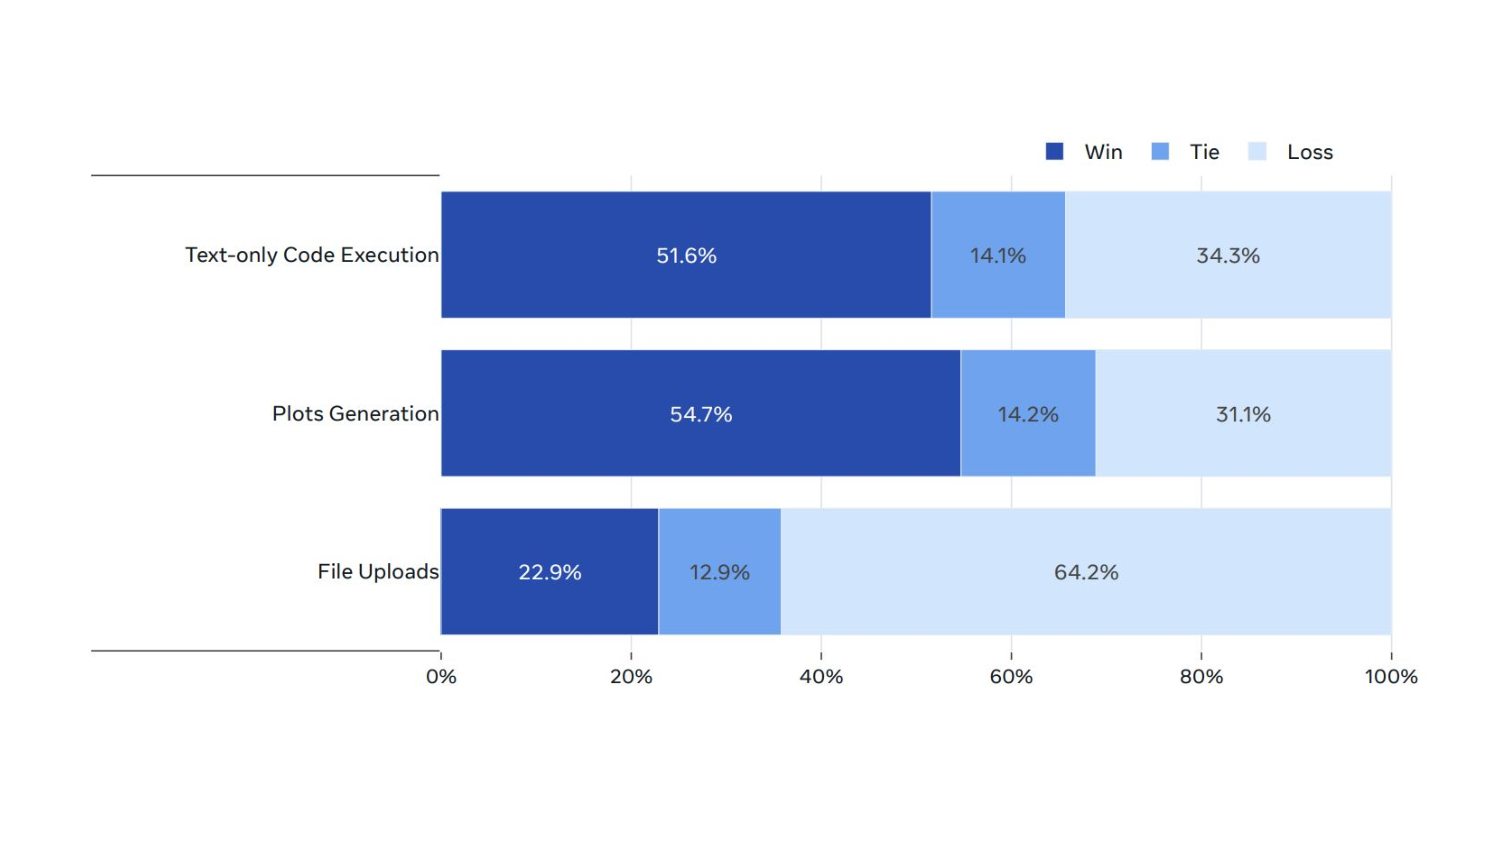
\includegraphics[width=0.75\linewidth]{assets/tool_human_evals.pdf}
    \caption{\textbf{Human evaluation results for \llamathree 405B vs. \gpto on code execution tasks including plotting and file uploads.} \llamathree 405B outperforms \gpto on code execution (without plotting or file uploads) as well as plot generation, but lags behind in file upload use cases.}
    \label{fig:heval-tool-win-rate}
\end{figure}

\textbf{Evaluation process.}
To perform a pairwise human evaluation of two models, we ask human annotators which of two model responses (produced by different models) they prefer.
Annotators use a 7-point scale for their ratings, enabling them to indicate whether one model response is much better than, better than, slightly better than, or about the same as the other model response.
When an annotator indicates that one model response is better or much better than the other model response, we consider this a ``win'' for that model.
We perform pairwise comparisons between models in which we report win rates per capability in the prompt set.

\textbf{Results.}
We use our human evaluation process to compare \llamathree 405B with GPT-4 (0125 API version), GPT-4o (API version), and Claude 3.5 Sonnet (API version).
The results of these evaluations are presented in Figure~\ref{fig:human_evaluation_results}.
We observe that \llamathree 405B performs approximately on par with the 0125 API version of GPT-4,
while achieving mixed results (some wins and some losses) compared to GPT-4o and Claude 3.5 Sonnet.
On nearly all capabilities, the win rates of \llamathree and GPT-4 are within the margin of error.
On multiturn reasoning and coding tasks, \llamathree 405B outperforms GPT-4 but it underperforms GPT-4 on multilingual (Hindi, Spanish, and Portuguese) prompts.
\llamathree performs on par with GPT-4o on English prompts, on par with Claude 3.5 Sonnet on multilingual prompts, and outperforms Claude 3.5 Sonnet on single and multiturn English prompts.
However, it trails Claude 3.5 Sonnet in capabilities such as coding and reasoning.
Qualitatively, we find that model performance in human evaluations is heavily influenced by nuanced factors such as model tone, response structure, and verbosity -- factors that we are optimizing for in our post-training process.
Overall, our human evaluation results are consistent with those on standard benchmark evaluations: \llamathree 405B is very competitive with leading industry models, making it the best-performing openly available model.



\begin{figure}[t]
    \centering
    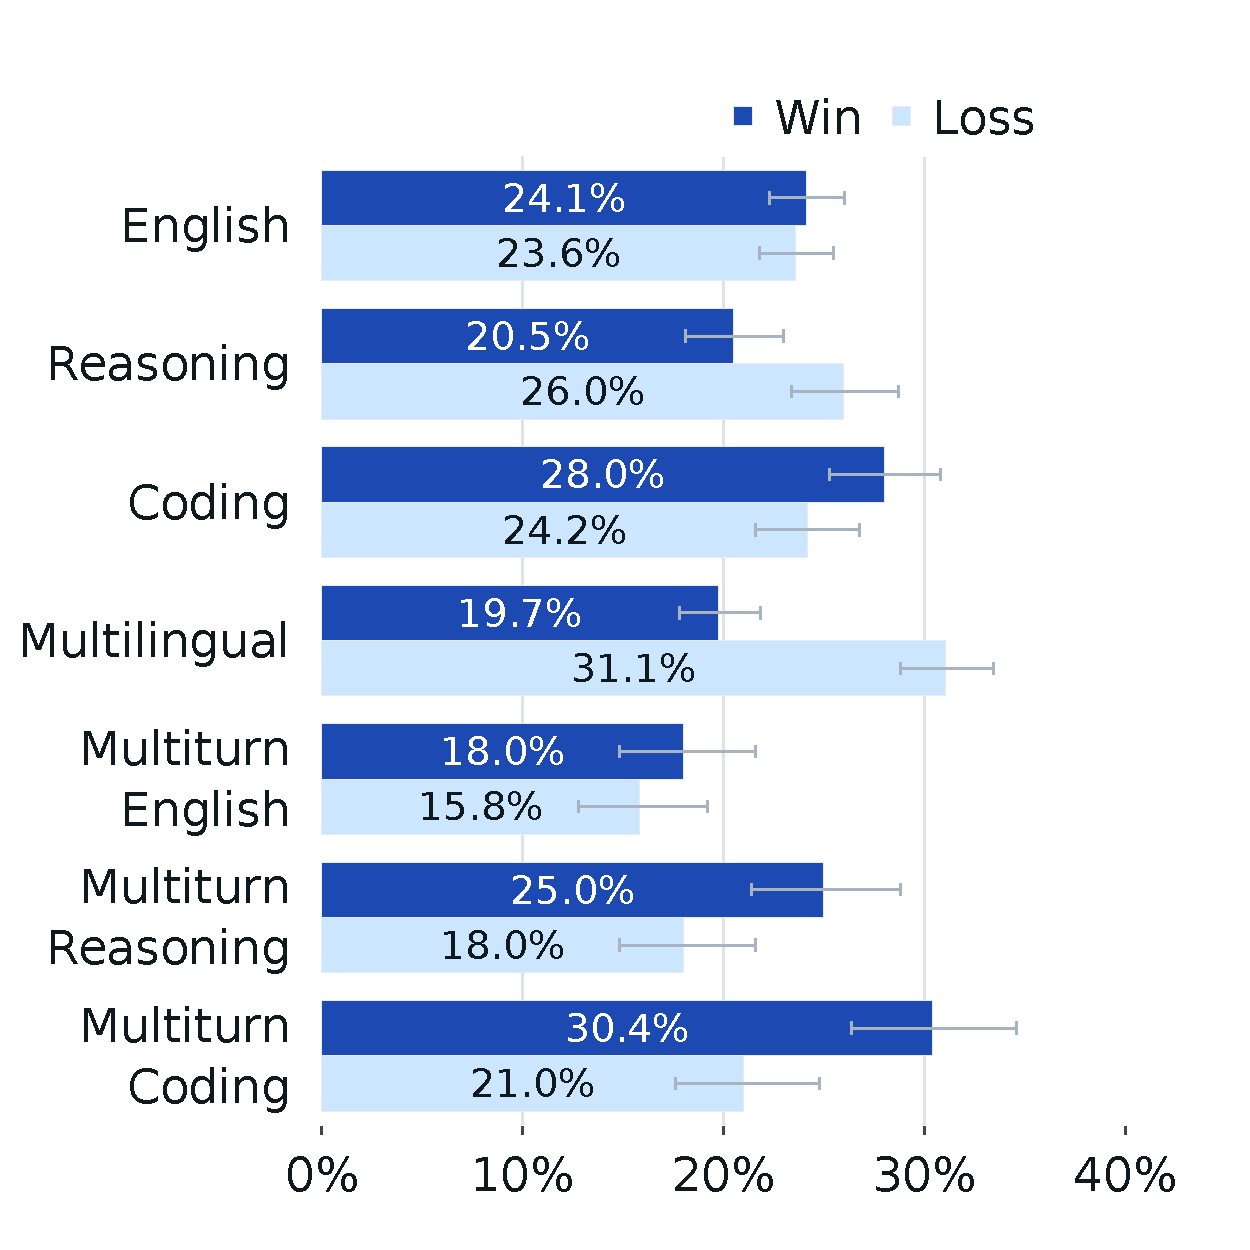
\includegraphics[height=0.38\linewidth]{assets/heval-gpt4preview-overall.pdf}\hspace{-0.03\linewidth}
    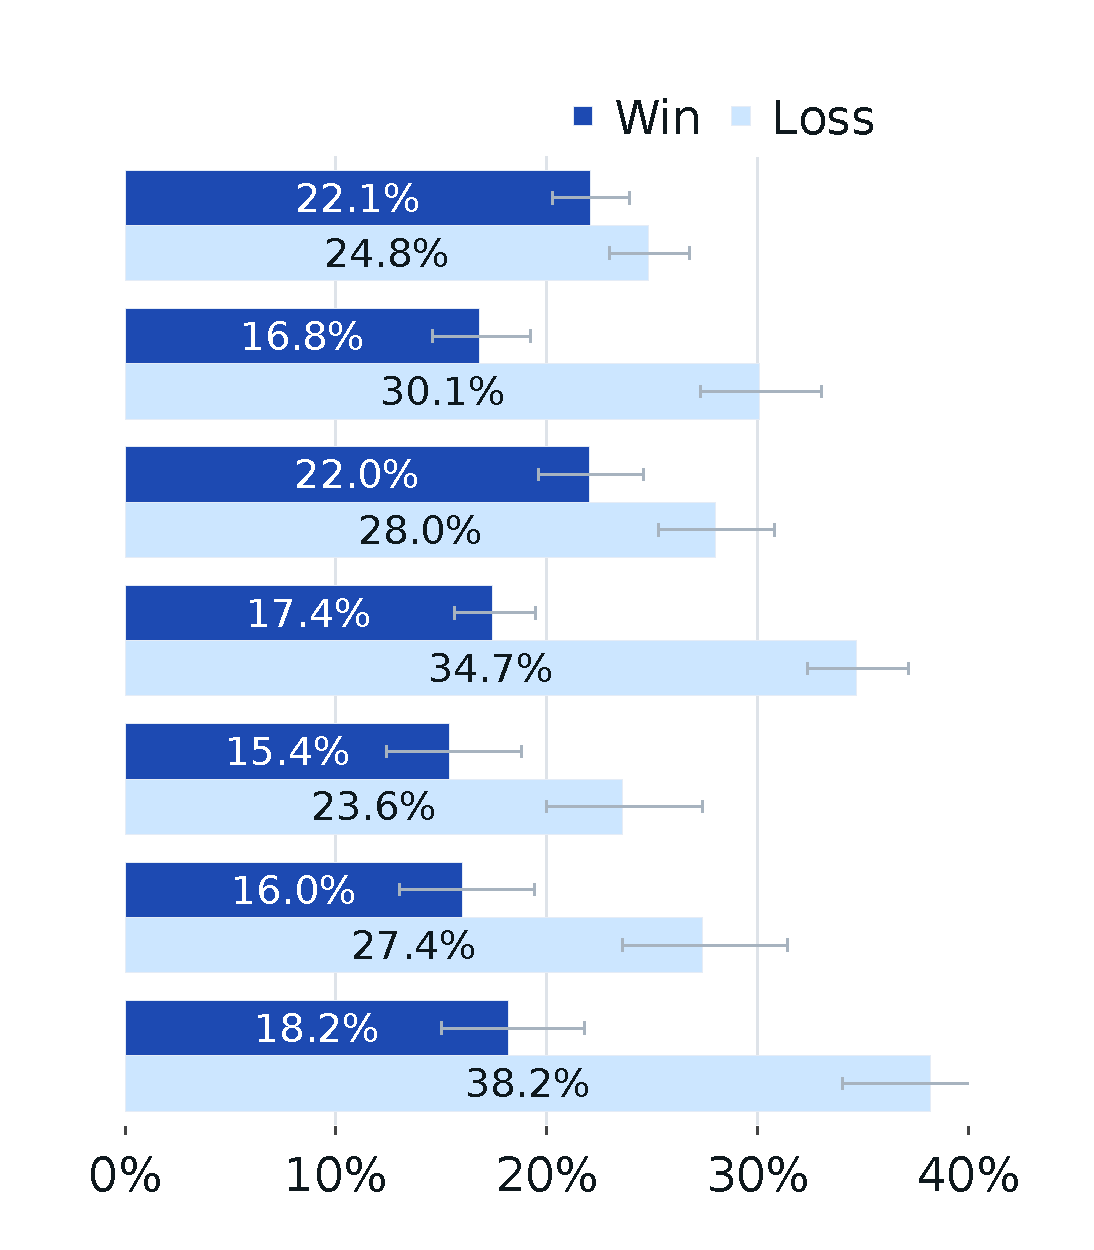
\includegraphics[height=0.38\linewidth]{assets/heval-gpt4o-overall.pdf}\hspace{-0.03\linewidth}
    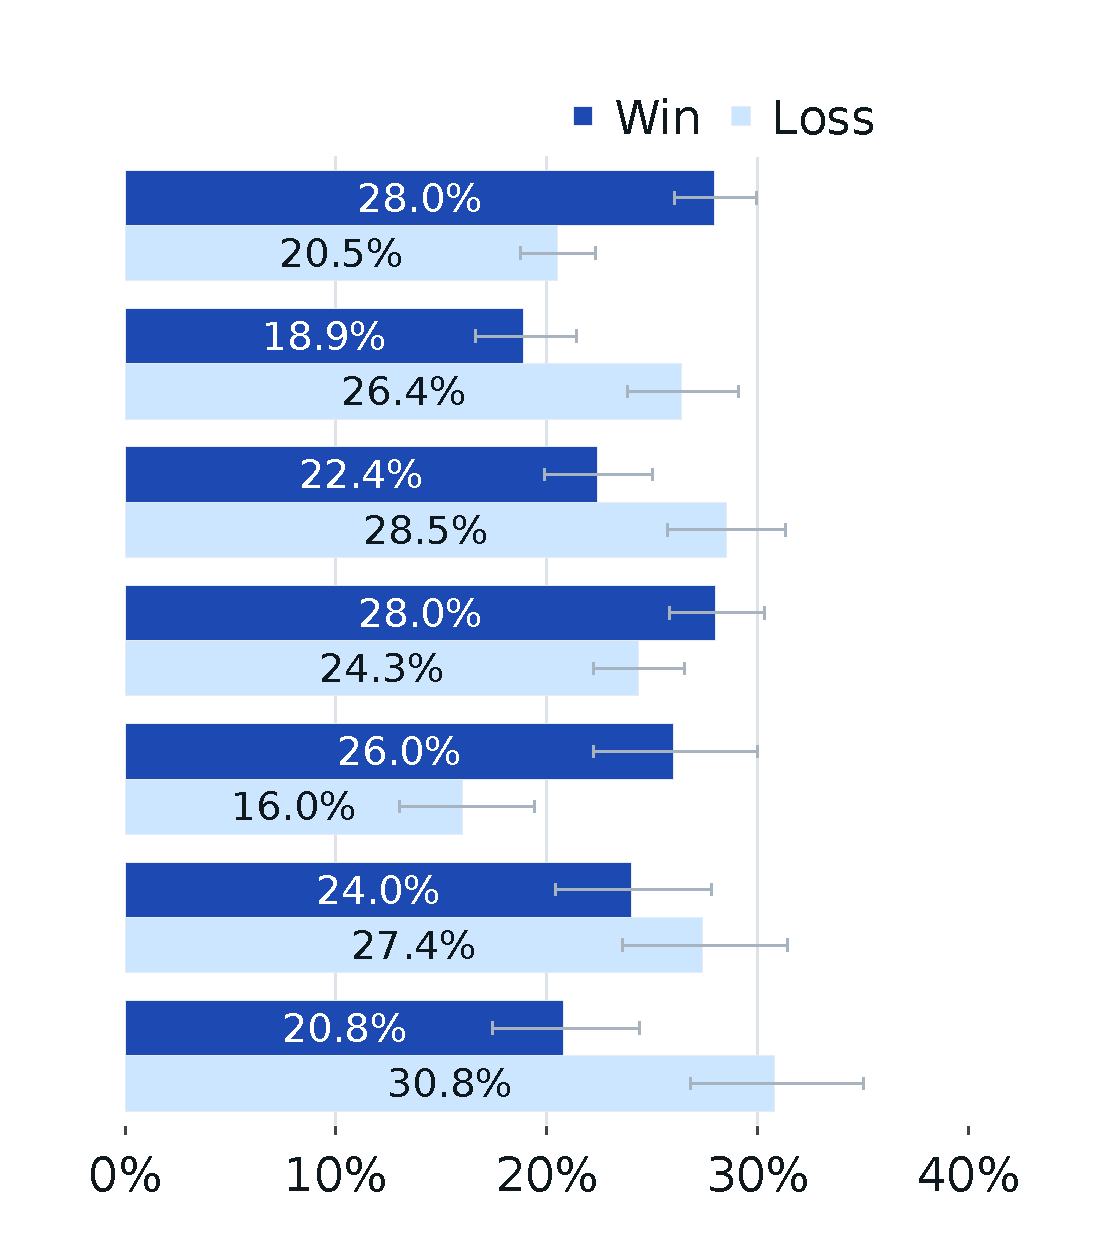
\includegraphics[height=0.38\linewidth]{assets/heval-claude3.5sonnet-overall.pdf}
    \caption{\textbf{Human evaluation results for the \llamathree 405B model.} \emph{Left:} Comparison with GPT-4. \emph{Middle:} Comparison with GPT-4o. \emph{Right:} Comparison with Claude 3.5 Sonnet. All results include 95\% confidence intervals and exclude ties.}
    \label{fig:human_evaluation_results}
\end{figure}

\textbf{Limitations.} All human evaluation results underwent a thorough data quality assurance process.
However, since it is challenging to define objective criteria for evaluating model responses, human evaluations can still be influenced by personal biases, backgrounds, and preferences of human annotators, which may lead to inconsistent or unreliable results.
